\documentclass[12pt]{article}
\usepackage{fancyhdr}
\pagestyle{fancy}
\fancyhf{}
\fancyfoot[C]{\thepage}
\fancyfoot[L]{\scriptsize CC BY-NC-SA 4.0 \textbullet\ Leo Liang}
\renewcommand{\headrulewidth}{0pt}
\usepackage[margin=1in]{geometry}
\usepackage{amsmath, amssymb}
\usepackage{array, booktabs}
\usepackage{pgffor}
\usepackage{tikz}
\parindent=0pt
\parskip=1em
\newcolumntype{C}[1]{>{\centering\arraybackslash}p{#1}}
\newcommand{\wl}{\par\vspace{5mm}\noindent\rule{\linewidth}{0.4pt}\par\vspace{1mm}}
\newcommand{\wls}[1]{\foreach \i in {1,...,#1}{\wl}}
\newcommand{\gridaxes}[1]{%
  \draw[step=1,gray!25,very thin] (-#1,-#1) grid (#1,#1);%
  \draw[thick,->] (-#1-0.4,0)--(#1+0.4,0) node[right]{\scriptsize$x$};%
  \draw[thick,->] (0,-#1-0.4)--(0,#1+0.4) node[above]{\scriptsize$y$};%
  \foreach \n in {-#1,...,#1}{\ifnum\n=0\else
      \draw (\n,0.07)--(\n,-0.07) node[below]{\tiny$\n$};
      \draw (0.07,\n)--(-0.07,\n) node[left]{\tiny$\n$};\fi}%
}
\newcommand{\blankgrid}[2][0.5]{%
  \begin{tikzpicture}[scale=#1]\gridaxes{#2}\end{tikzpicture}}
% ─────────────────────────────────────────────────────────────────────────────
\begin{document}
\pagestyle{fancy}
\begin{center}
  {\Large\bfseries Warm-Up Check --- Graphing Quadratics}\\[4pt]
  Name: \;\underline{\hspace{4cm}}\quad Date: \; \underline{\hspace{4cm}}
\end{center}
\hrule\bigskip

Show your work. This is just a check-in, not a test.

% ===========================================================================
\subsection*{Graph each quadratic}
Mark the vertex, then plot enough points to show the shape.

\medskip
\begin{minipage}[t]{0.48\linewidth}
\textbf{1.}\quad $y=-(x+2)^2+3$\\[2pt]
\centering\blankgrid[0.575]{5}
\end{minipage}\hfill
\begin{minipage}[t]{0.48\linewidth}
\textbf{2.}\quad $y=2(x-3)^2-4$\\[2pt]
\centering\blankgrid[0.575]{5}
\end{minipage}

% ===========================================================================
\newpage
\subsection*{Write the equation of each graph}
Each is a parabola $y=a(x-h)^2+k$. Read off the vertex, use one more point, and write the equation.

\medskip
% Q3: y=(3/4)(x-2)^2-3, vertex (2,-3), through (0,0) and (4,0)
\begin{minipage}[t]{0.48\linewidth}
\textbf{3.}\\[2pt]
\centering
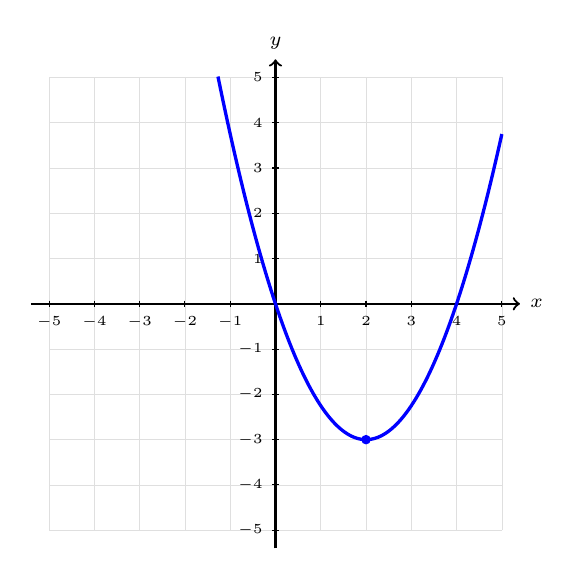
\begin{tikzpicture}[scale=0.575]
  \gridaxes{5}
  \draw[very thick,blue,domain=-1.27:5,samples=120] plot(\x,{(3/4)*(\x-2)^2-3});
  \fill[blue] (2,-3) circle (3pt);
\end{tikzpicture}
\par\vspace{9mm}\raggedright Equation: \underline{\hspace{4.5cm}}
\end{minipage}\hfill
% Q4: y=-(1/4)(x-1)^2+4, vertex (1,4), through (-1,3) and (3,3)
\begin{minipage}[t]{0.48\linewidth}
\textbf{4.}\\[2pt]
\centering
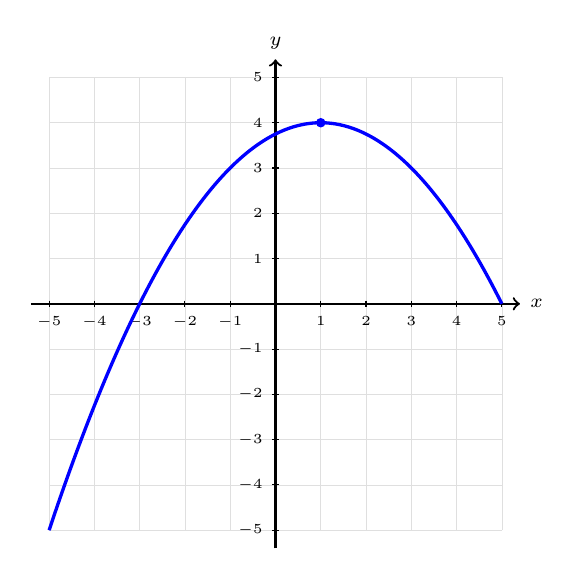
\begin{tikzpicture}[scale=0.575]
  \gridaxes{5}
  \draw[very thick,blue,domain=-5:5,samples=150] plot(\x,{-(1/4)*(\x-1)^2+4});
  \fill[blue] (1,4) circle (3pt);
\end{tikzpicture}
\par\vspace{9mm}\raggedright Equation: \underline{\hspace{4.5cm}}
\end{minipage}

% ===========================================================================
\newpage
\subsection*{Complete the square}
Write each in the form $a(x-h)^2+k$. Show your steps.

\bigskip
\textbf{5.}\quad $x^2 - 6x + 4$

\vspace{5cm}
\textbf{6.}\quad $2x^2 + 8x + 3$

\vspace{5cm}

% ===========================================================================
\newpage
\subsection*{Putting it together}
\textbf{7.}\quad For $\;y = x^2 + 2x + 3$:\quad complete the square to get vertex form, then graph it.

\vspace{4.5cm}
Vertex form: \underline{\hspace{4.5cm}}
\begin{center}\blankgrid[0.6]{6}\end{center}

% ===========================================================================
\end{document}